\documentclass[tikz,border=2pt]{standalone}
\usepackage{tikz}

\begin{document}
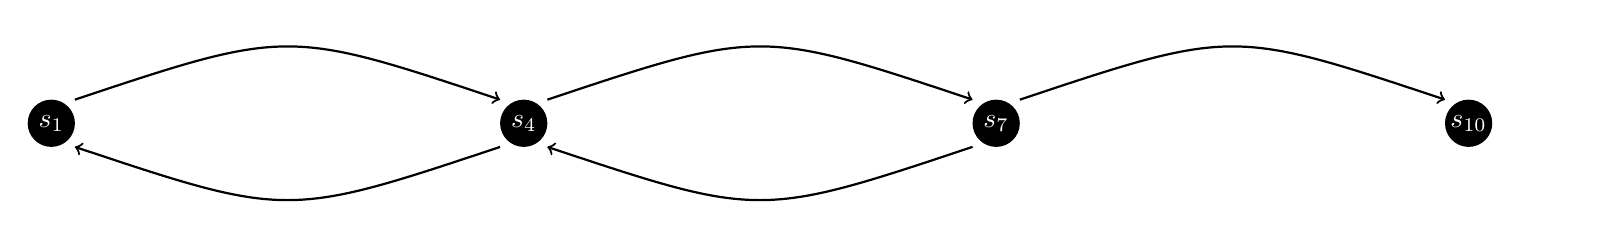
\begin{tikzpicture}[scale=2.0]

\def\r{0.15};
\def\n{10};
\foreach \x in {1,4,7,10}{
       \fill[fill=black] (\x, 0) circle [radius=\r];
       \node[white] at (\x, 0) {$s_{\x}$};
}

\fill[fill=white] (\n+0.5, 0) circle [radius=\r];
\foreach \x in {1,4,7}{
       \draw [black, thick, ->] (\x+\r, \r) .. controls (\x+1.5, 0.6) .. (\x+3-\r, \r);
       }
\foreach \x in {1,4}{
       \draw [black, thick, <-] (\x+\r, -\r) .. controls (\x+1.5, -0.6) .. (\x+3-\r, -\r);
}

\end{tikzpicture}
\end{document}
